\documentclass[]{article}
\usepackage{lmodern}
\usepackage{amssymb,amsmath}
\usepackage{ifxetex,ifluatex}
\usepackage{fixltx2e} % provides \textsubscript
\ifnum 0\ifxetex 1\fi\ifluatex 1\fi=0 % if pdftex
  \usepackage[T1]{fontenc}
  \usepackage[utf8]{inputenc}
\else % if luatex or xelatex
  \ifxetex
    \usepackage{mathspec}
  \else
    \usepackage{fontspec}
  \fi
  \defaultfontfeatures{Ligatures=TeX,Scale=MatchLowercase}
\fi
% use upquote if available, for straight quotes in verbatim environments
\IfFileExists{upquote.sty}{\usepackage{upquote}}{}
% use microtype if available
\IfFileExists{microtype.sty}{%
\usepackage{microtype}
\UseMicrotypeSet[protrusion]{basicmath} % disable protrusion for tt fonts
}{}
\usepackage[margin=1in]{geometry}
\usepackage{hyperref}
\hypersetup{unicode=true,
            pdftitle={Reproducible Research : Project-2},
            pdfborder={0 0 0},
            breaklinks=true}
\urlstyle{same}  % don't use monospace font for urls
\usepackage{color}
\usepackage{fancyvrb}
\newcommand{\VerbBar}{|}
\newcommand{\VERB}{\Verb[commandchars=\\\{\}]}
\DefineVerbatimEnvironment{Highlighting}{Verbatim}{commandchars=\\\{\}}
% Add ',fontsize=\small' for more characters per line
\usepackage{framed}
\definecolor{shadecolor}{RGB}{248,248,248}
\newenvironment{Shaded}{\begin{snugshade}}{\end{snugshade}}
\newcommand{\AlertTok}[1]{\textcolor[rgb]{0.94,0.16,0.16}{#1}}
\newcommand{\AnnotationTok}[1]{\textcolor[rgb]{0.56,0.35,0.01}{\textbf{\textit{#1}}}}
\newcommand{\AttributeTok}[1]{\textcolor[rgb]{0.77,0.63,0.00}{#1}}
\newcommand{\BaseNTok}[1]{\textcolor[rgb]{0.00,0.00,0.81}{#1}}
\newcommand{\BuiltInTok}[1]{#1}
\newcommand{\CharTok}[1]{\textcolor[rgb]{0.31,0.60,0.02}{#1}}
\newcommand{\CommentTok}[1]{\textcolor[rgb]{0.56,0.35,0.01}{\textit{#1}}}
\newcommand{\CommentVarTok}[1]{\textcolor[rgb]{0.56,0.35,0.01}{\textbf{\textit{#1}}}}
\newcommand{\ConstantTok}[1]{\textcolor[rgb]{0.00,0.00,0.00}{#1}}
\newcommand{\ControlFlowTok}[1]{\textcolor[rgb]{0.13,0.29,0.53}{\textbf{#1}}}
\newcommand{\DataTypeTok}[1]{\textcolor[rgb]{0.13,0.29,0.53}{#1}}
\newcommand{\DecValTok}[1]{\textcolor[rgb]{0.00,0.00,0.81}{#1}}
\newcommand{\DocumentationTok}[1]{\textcolor[rgb]{0.56,0.35,0.01}{\textbf{\textit{#1}}}}
\newcommand{\ErrorTok}[1]{\textcolor[rgb]{0.64,0.00,0.00}{\textbf{#1}}}
\newcommand{\ExtensionTok}[1]{#1}
\newcommand{\FloatTok}[1]{\textcolor[rgb]{0.00,0.00,0.81}{#1}}
\newcommand{\FunctionTok}[1]{\textcolor[rgb]{0.00,0.00,0.00}{#1}}
\newcommand{\ImportTok}[1]{#1}
\newcommand{\InformationTok}[1]{\textcolor[rgb]{0.56,0.35,0.01}{\textbf{\textit{#1}}}}
\newcommand{\KeywordTok}[1]{\textcolor[rgb]{0.13,0.29,0.53}{\textbf{#1}}}
\newcommand{\NormalTok}[1]{#1}
\newcommand{\OperatorTok}[1]{\textcolor[rgb]{0.81,0.36,0.00}{\textbf{#1}}}
\newcommand{\OtherTok}[1]{\textcolor[rgb]{0.56,0.35,0.01}{#1}}
\newcommand{\PreprocessorTok}[1]{\textcolor[rgb]{0.56,0.35,0.01}{\textit{#1}}}
\newcommand{\RegionMarkerTok}[1]{#1}
\newcommand{\SpecialCharTok}[1]{\textcolor[rgb]{0.00,0.00,0.00}{#1}}
\newcommand{\SpecialStringTok}[1]{\textcolor[rgb]{0.31,0.60,0.02}{#1}}
\newcommand{\StringTok}[1]{\textcolor[rgb]{0.31,0.60,0.02}{#1}}
\newcommand{\VariableTok}[1]{\textcolor[rgb]{0.00,0.00,0.00}{#1}}
\newcommand{\VerbatimStringTok}[1]{\textcolor[rgb]{0.31,0.60,0.02}{#1}}
\newcommand{\WarningTok}[1]{\textcolor[rgb]{0.56,0.35,0.01}{\textbf{\textit{#1}}}}
\usepackage{graphicx,grffile}
\makeatletter
\def\maxwidth{\ifdim\Gin@nat@width>\linewidth\linewidth\else\Gin@nat@width\fi}
\def\maxheight{\ifdim\Gin@nat@height>\textheight\textheight\else\Gin@nat@height\fi}
\makeatother
% Scale images if necessary, so that they will not overflow the page
% margins by default, and it is still possible to overwrite the defaults
% using explicit options in \includegraphics[width, height, ...]{}
\setkeys{Gin}{width=\maxwidth,height=\maxheight,keepaspectratio}
\IfFileExists{parskip.sty}{%
\usepackage{parskip}
}{% else
\setlength{\parindent}{0pt}
\setlength{\parskip}{6pt plus 2pt minus 1pt}
}
\setlength{\emergencystretch}{3em}  % prevent overfull lines
\providecommand{\tightlist}{%
  \setlength{\itemsep}{0pt}\setlength{\parskip}{0pt}}
\setcounter{secnumdepth}{0}
% Redefines (sub)paragraphs to behave more like sections
\ifx\paragraph\undefined\else
\let\oldparagraph\paragraph
\renewcommand{\paragraph}[1]{\oldparagraph{#1}\mbox{}}
\fi
\ifx\subparagraph\undefined\else
\let\oldsubparagraph\subparagraph
\renewcommand{\subparagraph}[1]{\oldsubparagraph{#1}\mbox{}}
\fi

%%% Use protect on footnotes to avoid problems with footnotes in titles
\let\rmarkdownfootnote\footnote%
\def\footnote{\protect\rmarkdownfootnote}

%%% Change title format to be more compact
\usepackage{titling}

% Create subtitle command for use in maketitle
\providecommand{\subtitle}[1]{
  \posttitle{
    \begin{center}\large#1\end{center}
    }
}

\setlength{\droptitle}{-2em}

  \title{Reproducible Research : Project-2}
    \pretitle{\vspace{\droptitle}\centering\huge}
  \posttitle{\par}
    \author{}
    \preauthor{}\postauthor{}
    \date{}
    \predate{}\postdate{}
  

\begin{document}
\maketitle

\hypertarget{executive-summary}{%
\subsubsection{Executive Summary}\label{executive-summary}}

\hypertarget{in-this-report-we-look-at-a-data-set-of-a-collection-of-car-and-are-interested-in-exploring-the-relationship-between-a-set-of-variables-and-miles-per-gallon-mpg-outcome.-particularly-we-are-interested-in-the-following-two-questions}{%
\paragraph{In this report, we look at a data set of a collection of car,
and are interested in exploring the relationship between a set of
variables and miles per gallon (MPG) (outcome). Particularly, we are
interested in the following two
questions:}\label{in-this-report-we-look-at-a-data-set-of-a-collection-of-car-and-are-interested-in-exploring-the-relationship-between-a-set-of-variables-and-miles-per-gallon-mpg-outcome.-particularly-we-are-interested-in-the-following-two-questions}}

\begin{verbatim}
* “Is an automatic or manual transmission better for MPG”
* “Quantify the MPG difference between automatic and manual transmissions”
\end{verbatim}

\hypertarget{in-order-to-answer-these-two-questions-we-follow-the-steps-below}{%
\paragraph{In order to answer these two questions, we follow the steps
below:}\label{in-order-to-answer-these-two-questions-we-follow-the-steps-below}}

\begin{verbatim}
* Load and process the data such that it makes more sense
* Conduct a basic exploratory data analyses to show the relationship between mpg and am
* Fit multiple models to the data and select the best model
* Diagnose the model and quantify the uncertainty
* Using the model we choose, draw conclusion and answer the questions
\end{verbatim}

\hypertarget{load-and-process-the-data}{%
\subsection{Load and Process the Data}\label{load-and-process-the-data}}

\hypertarget{load-the-mtcars-dataset-and-have-a-overview-of-it.}{%
\paragraph{Load the mtcars dataset and have a overview of
it.}\label{load-the-mtcars-dataset-and-have-a-overview-of-it.}}

\begin{Shaded}
\begin{Highlighting}[]
\KeywordTok{library}\NormalTok{(ggplot2)}
\end{Highlighting}
\end{Shaded}

\begin{verbatim}
## Registered S3 methods overwritten by 'ggplot2':
##   method         from 
##   [.quosures     rlang
##   c.quosures     rlang
##   print.quosures rlang
\end{verbatim}

\begin{Shaded}
\begin{Highlighting}[]
\KeywordTok{data}\NormalTok{(mtcars)}
\KeywordTok{head}\NormalTok{(mtcars)}
\end{Highlighting}
\end{Shaded}

\begin{verbatim}
##                    mpg cyl disp  hp drat    wt  qsec vs am gear carb
## Mazda RX4         21.0   6  160 110 3.90 2.620 16.46  0  1    4    4
## Mazda RX4 Wag     21.0   6  160 110 3.90 2.875 17.02  0  1    4    4
## Datsun 710        22.8   4  108  93 3.85 2.320 18.61  1  1    4    1
## Hornet 4 Drive    21.4   6  258 110 3.08 3.215 19.44  1  0    3    1
## Hornet Sportabout 18.7   8  360 175 3.15 3.440 17.02  0  0    3    2
## Valiant           18.1   6  225 105 2.76 3.460 20.22  1  0    3    1
\end{verbatim}

\hypertarget{change-some-variables-to-factor-since-they-represent-categories-not-continuous-values.}{%
\paragraph{Change some variables to factor since they represent
categories not continuous
values.}\label{change-some-variables-to-factor-since-they-represent-categories-not-continuous-values.}}

\begin{Shaded}
\begin{Highlighting}[]
\NormalTok{mtcars}\OperatorTok{$}\NormalTok{cyl <-}\StringTok{ }\KeywordTok{as.factor}\NormalTok{(mtcars}\OperatorTok{$}\NormalTok{cyl)}
\NormalTok{mtcars}\OperatorTok{$}\NormalTok{vs <-}\StringTok{ }\KeywordTok{as.factor}\NormalTok{(mtcars}\OperatorTok{$}\NormalTok{vs)}
\NormalTok{mtcars}\OperatorTok{$}\NormalTok{am <-}\StringTok{ }\KeywordTok{factor}\NormalTok{(mtcars}\OperatorTok{$}\NormalTok{am)}
\KeywordTok{levels}\NormalTok{(mtcars}\OperatorTok{$}\NormalTok{am) <-}\StringTok{ }\KeywordTok{c}\NormalTok{(}\StringTok{"automatic"}\NormalTok{, }\StringTok{"manual"}\NormalTok{)}
\NormalTok{mtcars}\OperatorTok{$}\NormalTok{gear <-}\StringTok{ }\KeywordTok{factor}\NormalTok{(mtcars}\OperatorTok{$}\NormalTok{gear)}
\NormalTok{mtcars}\OperatorTok{$}\NormalTok{carb <-}\StringTok{ }\KeywordTok{factor}\NormalTok{(mtcars}\OperatorTok{$}\NormalTok{carb)}
\end{Highlighting}
\end{Shaded}

\hypertarget{exploratory-analyses}{%
\subsection{Exploratory Analyses}\label{exploratory-analyses}}

\hypertarget{we-are-interested-in-the-relationship-between-mpg-miles-per-gallon-and-am-transmission-so-lets-take-a-look.}{%
\paragraph{We are interested in the relationship between mpg (miles per
gallon) and am (transmission), so let's take a
look.}\label{we-are-interested-in-the-relationship-between-mpg-miles-per-gallon-and-am-transmission-so-lets-take-a-look.}}

\begin{Shaded}
\begin{Highlighting}[]
\KeywordTok{boxplot}\NormalTok{(mpg }\OperatorTok{~}\StringTok{ }\NormalTok{am, }\DataTypeTok{data =}\NormalTok{ mtcars, }\DataTypeTok{xlab =} \StringTok{"Transmission (0 = automatic, 1 = manual)"}\NormalTok{)}
\end{Highlighting}
\end{Shaded}

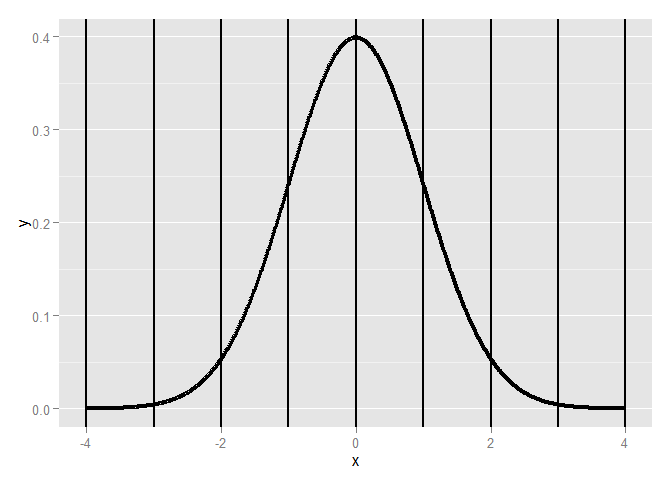
\includegraphics{Regression_Models_Course_Project_files/figure-latex/unnamed-chunk-3-1.pdf}

\hypertarget{box-plot-clearly-shows-that-theres-a-good-separation-between-two-groups-and-cars-with-manual-transmission-have-higher-mpg-than-cars-with-automatice-transmission.}{%
\paragraph{Box plot clearly shows that there's a good separation between
two groups, and cars with manual transmission have higher mpg than cars
with automatice
transmission.}\label{box-plot-clearly-shows-that-theres-a-good-separation-between-two-groups-and-cars-with-manual-transmission-have-higher-mpg-than-cars-with-automatice-transmission.}}

\hypertarget{statistical-inference}{%
\subsection{Statistical Inference}\label{statistical-inference}}

\hypertarget{we-can-also-conduct-a-t-test-to-confirm-our-observation.-define-the-null-hypothesis-as-manual-and-automatic-transmissions-result-in-the-same-mpg.}{%
\paragraph{We can also conduct a T-test to confirm our observation.
Define the null hypothesis as manual and automatic transmissions result
in the same
mpg.}\label{we-can-also-conduct-a-t-test-to-confirm-our-observation.-define-the-null-hypothesis-as-manual-and-automatic-transmissions-result-in-the-same-mpg.}}

\begin{Shaded}
\begin{Highlighting}[]
\KeywordTok{t.test}\NormalTok{(mpg }\OperatorTok{~}\StringTok{ }\NormalTok{am, }\DataTypeTok{data =}\NormalTok{ mtcars)}
\end{Highlighting}
\end{Shaded}

\begin{verbatim}
## 
##  Welch Two Sample t-test
## 
## data:  mpg by am
## t = -3.7671, df = 18.332, p-value = 0.001374
## alternative hypothesis: true difference in means is not equal to 0
## 95 percent confidence interval:
##  -11.280194  -3.209684
## sample estimates:
## mean in group automatic    mean in group manual 
##                17.14737                24.39231
\end{verbatim}

\hypertarget{p-value-is-0.00137-and-confidence-interval-does-not-include-zero-so-we-reject-the-null-hypothesis-and-accept-the-difference-in-mpg-between-manual-and-automatic-transmission-which-we-observed-earlier.}{%
\paragraph{P-value is 0.00137, and confidence interval does not include
zero, so we reject the null hypothesis and accept the difference in mpg
between manual and automatic transmission, which we observed
earlier.}\label{p-value-is-0.00137-and-confidence-interval-does-not-include-zero-so-we-reject-the-null-hypothesis-and-accept-the-difference-in-mpg-between-manual-and-automatic-transmission-which-we-observed-earlier.}}

\hypertarget{regression-models}{%
\subsection{Regression Models}\label{regression-models}}

\hypertarget{simple-model}{%
\subsubsection{Simple Model}\label{simple-model}}

\hypertarget{first-we-use-the-simplest-model-with-mpg-as-outcome-and-am-as-predictor.}{%
\paragraph{First we use the simplest model with mpg as outcome and am as
predictor.}\label{first-we-use-the-simplest-model-with-mpg-as-outcome-and-am-as-predictor.}}

\begin{Shaded}
\begin{Highlighting}[]
\NormalTok{simpleMod <-}\StringTok{ }\KeywordTok{lm}\NormalTok{(mpg }\OperatorTok{~}\StringTok{ }\NormalTok{am, mtcars)}
\KeywordTok{summary}\NormalTok{(simpleMod)}
\end{Highlighting}
\end{Shaded}

\begin{verbatim}
## 
## Call:
## lm(formula = mpg ~ am, data = mtcars)
## 
## Residuals:
##     Min      1Q  Median      3Q     Max 
## -9.3923 -3.0923 -0.2974  3.2439  9.5077 
## 
## Coefficients:
##             Estimate Std. Error t value Pr(>|t|)    
## (Intercept)   17.147      1.125  15.247 1.13e-15 ***
## ammanual       7.245      1.764   4.106 0.000285 ***
## ---
## Signif. codes:  0 '***' 0.001 '**' 0.01 '*' 0.05 '.' 0.1 ' ' 1
## 
## Residual standard error: 4.902 on 30 degrees of freedom
## Multiple R-squared:  0.3598, Adjusted R-squared:  0.3385 
## F-statistic: 16.86 on 1 and 30 DF,  p-value: 0.000285
\end{verbatim}

\hypertarget{this-shows-that-cars-with-automatic-transmission-have-17.147-average-mpg-whereas-cars-with-manual-transmission-have-averagely-7.245-mpg-higher.-the-p-values-are-very-low-but-the-r-squared-value-is-0.3385-which-means-that-the-model-can-only-explain-33.85-of-the-mpg-variance.-therefore-we-need-to-take-more-variables-into-consideration.}{%
\paragraph{This shows that cars with automatic transmission have 17.147
average mpg, whereas cars with manual transmission have averagely 7.245
mpg higher. The p-values are very low, but the R-squared value is
0.3385, which means that the model can only explain 33.85\% of the mpg
variance. Therefore, we need to take more variables into
consideration.}\label{this-shows-that-cars-with-automatic-transmission-have-17.147-average-mpg-whereas-cars-with-manual-transmission-have-averagely-7.245-mpg-higher.-the-p-values-are-very-low-but-the-r-squared-value-is-0.3385-which-means-that-the-model-can-only-explain-33.85-of-the-mpg-variance.-therefore-we-need-to-take-more-variables-into-consideration.}}

\hypertarget{full-model}{%
\subsection{Full Model}\label{full-model}}

\hypertarget{we-then-fit-all-variables-into-the-model.}{%
\paragraph{We then fit all variables into the
model.}\label{we-then-fit-all-variables-into-the-model.}}

\begin{Shaded}
\begin{Highlighting}[]
\NormalTok{fullMod <-}\StringTok{ }\KeywordTok{lm}\NormalTok{(mpg }\OperatorTok{~}\StringTok{ }\NormalTok{., mtcars)}
\KeywordTok{summary}\NormalTok{(fullMod)}
\end{Highlighting}
\end{Shaded}

\begin{verbatim}
## 
## Call:
## lm(formula = mpg ~ ., data = mtcars)
## 
## Residuals:
##     Min      1Q  Median      3Q     Max 
## -3.5087 -1.3584 -0.0948  0.7745  4.6251 
## 
## Coefficients:
##             Estimate Std. Error t value Pr(>|t|)  
## (Intercept) 23.87913   20.06582   1.190   0.2525  
## cyl6        -2.64870    3.04089  -0.871   0.3975  
## cyl8        -0.33616    7.15954  -0.047   0.9632  
## disp         0.03555    0.03190   1.114   0.2827  
## hp          -0.07051    0.03943  -1.788   0.0939 .
## drat         1.18283    2.48348   0.476   0.6407  
## wt          -4.52978    2.53875  -1.784   0.0946 .
## qsec         0.36784    0.93540   0.393   0.6997  
## vs1          1.93085    2.87126   0.672   0.5115  
## ammanual     1.21212    3.21355   0.377   0.7113  
## gear4        1.11435    3.79952   0.293   0.7733  
## gear5        2.52840    3.73636   0.677   0.5089  
## carb2       -0.97935    2.31797  -0.423   0.6787  
## carb3        2.99964    4.29355   0.699   0.4955  
## carb4        1.09142    4.44962   0.245   0.8096  
## carb6        4.47757    6.38406   0.701   0.4938  
## carb8        7.25041    8.36057   0.867   0.3995  
## ---
## Signif. codes:  0 '***' 0.001 '**' 0.01 '*' 0.05 '.' 0.1 ' ' 1
## 
## Residual standard error: 2.833 on 15 degrees of freedom
## Multiple R-squared:  0.8931, Adjusted R-squared:  0.779 
## F-statistic:  7.83 on 16 and 15 DF,  p-value: 0.000124
\end{verbatim}

\hypertarget{this-time-the-r-squared-value-0.8931-is-decent.-however-the-p-values-are-all-greater-than-5-and-hence-show-no-significance.-we-then-need-to-select-the-most-significant-variables.-this-can-be-done-by-backward-selection-using-step-function.}{%
\paragraph{This time the R-squared value 0.8931 is decent. However, the
p-values are all greater than 5\% and hence show no significance. We
then need to select the most significant variables. This can be done by
backward selection using step
function.}\label{this-time-the-r-squared-value-0.8931-is-decent.-however-the-p-values-are-all-greater-than-5-and-hence-show-no-significance.-we-then-need-to-select-the-most-significant-variables.-this-can-be-done-by-backward-selection-using-step-function.}}

\hypertarget{step-model}{%
\subsection{Step Model}\label{step-model}}

\hypertarget{the-resulting-model-is-mpg-wt-qsec-am-with-all-p-values-smaller-than-5-and-the-adjusted-r-squared-value-0.8336-which-accouts-for-83.36-of-the-variance-in-mpg.}{%
\paragraph{The resulting model is mpg \textasciitilde{} wt + qsec + am,
with all p-values smaller than 5\% and the adjusted R-squared value
0.8336 which accouts for 83.36\% of the variance in
mpg.}\label{the-resulting-model-is-mpg-wt-qsec-am-with-all-p-values-smaller-than-5-and-the-adjusted-r-squared-value-0.8336-which-accouts-for-83.36-of-the-variance-in-mpg.}}

\hypertarget{the-am-coefficient-indicates-that-holding-wt-and-qsec-constant-cars-with-manual-transmission-have-2.9358-more-mpg-than-cars-with-automatic-transmission-on-average.}{%
\paragraph{The am coefficient indicates that holding wt and qsec
constant, cars with manual transmission have 2.9358 more mpg than cars
with automatic transmission on
average.}\label{the-am-coefficient-indicates-that-holding-wt-and-qsec-constant-cars-with-manual-transmission-have-2.9358-more-mpg-than-cars-with-automatic-transmission-on-average.}}

\hypertarget{model-diagnosis}{%
\subsection{Model diagnosis}\label{model-diagnosis}}

\hypertarget{the-95-two-sided-confidence-interval-of-the-coefficients-are-as-follows}{%
\paragraph{The 95\% two-sided confidence interval of the coefficients
are as
follows:}\label{the-95-two-sided-confidence-interval-of-the-coefficients-are-as-follows}}

\begin{Shaded}
\begin{Highlighting}[]
\KeywordTok{confint}\NormalTok{(stepMod)}
\end{Highlighting}
\end{Shaded}

\begin{verbatim}
##                   2.5 %    97.5 %
## (Intercept) -4.63829946 23.873860
## wt          -5.37333423 -2.459673
## qsec         0.63457320  1.817199
## ammanual     0.04573031  5.825944
\end{verbatim}

\hypertarget{lets-plot-the-diagnosis-of-the-model.}{%
\paragraph{Let's plot the diagnosis of the
model.}\label{lets-plot-the-diagnosis-of-the-model.}}

\begin{Shaded}
\begin{Highlighting}[]
\KeywordTok{par}\NormalTok{(}\DataTypeTok{mfrow =} \KeywordTok{c}\NormalTok{(}\DecValTok{2}\NormalTok{, }\DecValTok{2}\NormalTok{))}
\KeywordTok{plot}\NormalTok{(stepMod)}
\end{Highlighting}
\end{Shaded}

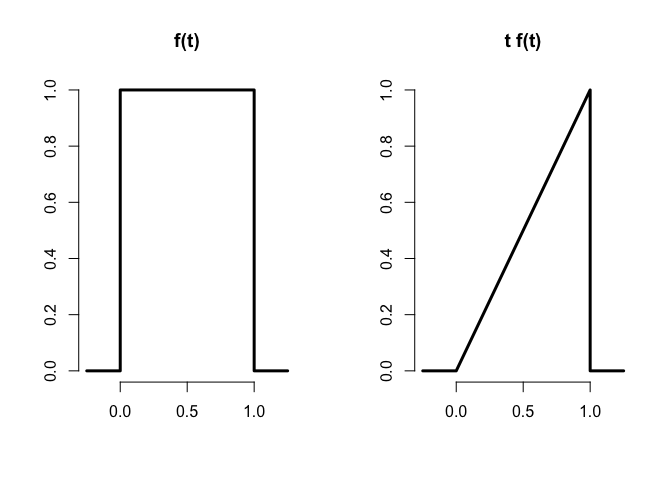
\includegraphics{Regression_Models_Course_Project_files/figure-latex/unnamed-chunk-8-1.pdf}

\hypertarget{conclusion}{%
\subsection{Conclusion}\label{conclusion}}

\hypertarget{from-the-above-analysis-we-can-conclude-that-a-manual-transmission-is-better-in-terms-of-mpg-than-an-automatic-transmission.-holding-weight-lb1000-and-qsec-14-mile-time-constant-a-manual-tranmission-has-averagely-2.9358-more-mpg-miles-per-gallon-than-an-automatic-transmission.}{%
\paragraph{From the above analysis, we can conclude that a manual
transmission is better in terms of MPG than an automatic transmission.
Holding weight (lb/1000) and qsec (1/4 mile time) constant, a manual
tranmission has averagely 2.9358 more MPG (miles per gallon) than an
automatic
transmission.}\label{from-the-above-analysis-we-can-conclude-that-a-manual-transmission-is-better-in-terms-of-mpg-than-an-automatic-transmission.-holding-weight-lb1000-and-qsec-14-mile-time-constant-a-manual-tranmission-has-averagely-2.9358-more-mpg-miles-per-gallon-than-an-automatic-transmission.}}


\end{document}
